\documentclass{article}

\usepackage{fancyhdr}
\usepackage{extramarks}
\usepackage{amsmath}
\usepackage{minted}
\usepackage{amsthm}
\usepackage{amsfonts}
\usepackage{tikz}
\usepackage{algorithm}
\usepackage{algpseudocode}
\usepackage{adjustbox}
\usepackage{graphicx}
\usetikzlibrary{automata,positioning}
\usepackage{fullpage,enumitem,amsmath,amssymb,graphicx}
\usepackage[sort]{natbib}
\usepackage[colorlinks=true,urlcolor=blue]{hyperref}        

%
% Basic Document Settings
%

\topmargin=-0.75in
\textwidth=6.5in
\textheight=9.0in
\headsep=0.20in
\headheight = 12pt
\linespread{1.1}

\pagestyle{fancy}
\chead{\hmwkClass\ (\hmwkClassInstructor): \hmwkTitle}
\rhead{\firstxmark}
\lfoot{\lastxmark}
\cfoot{\thepage}

\renewcommand\headrulewidth{0.55pt}
\renewcommand\footrulewidth{0.55pt}

\setlength\parindent{0pt}


\setcounter{secnumdepth}{0}

%
% Homework Problem Environment
%
% This environment takes an optional argument. When given, it will adjust the
% problem counter. This is useful for when the problems given for your
% assignment aren't sequential. See the last 3 problems of this template for an
% example.

%
% Homework Details
%   - Title
%   - Due date
%   - Class
%   - Section/Time
%   - Instructor
%   - Author
%

\newcommand{\hmwkTitle}{Homework\ \#1}
\newcommand{\hmwkDueDate}{October 11, 2021}
\newcommand{\hmwkClassCode}{COT 5405}
\newcommand{\hmwkClass}{Analysis of Algorithms}
\newcommand{\hmwkClassYear}{Fall 2021}
\newcommand{\hmwkClassInstructor}{Professor Alin Dobra}
\newcommand{\hmwkAuthorName}{\textit{Vyom Pathak}}
\newcommand{\hmwkUFID}{96703101}

%
%
%
% Various Helper Commands
%

% Useful for algorithms
\newcommand{\alg}[1]{\textsc{\bfseries \footnotesize #1}}

% For derivatives
\newcommand{\deriv}[1]{\frac{\mathrm{d}}{\mathrm{d}x} (#1)}

% For partial derivatives
\newcommand{\pderiv}[2]{\frac{\partial}{\partial #1} (#2)}

% Integral dx
\newcommand{\dx}{\mathrm{d}x}

% Alias for the Solution section header
\newcommand{\solution}{\textbf{\large Solution}}

% Probability commands: Expectation, Variance, Covariance, Bias
\newcommand{\E}{\mathrm{E}}
\newcommand{\Var}{\mathrm{Var}}
\newcommand{\Cov}{\mathrm{Cov}}
\newcommand{\Bias}{\mathrm{Bias}}

% norm bars
\newcommand{\norm}[1]{\left\lVert#1\right\rVert}

\begin{document}

\begin{center}
{\Large \hmwkClassCode\ \hmwkClass\ \hmwkClassYear\ \hmwkTitle}

\begin{tabular}{rl}
UFID: & \hmwkUFID \\
Name: & \hmwkAuthorName \\
Instructor: & \hmwkClassInstructor \\
Due Date: & \hmwkDueDate \\ 
% Collaborators: & [list all the people you worked with]
\end{tabular}
\end{center}

\section*{Problem 1}
\subsection*{Cycle Finding [50]}
\subsubsection*{Solution}
\textbf{Algorithm}\\
The algorithm to detect and find the cycle in given in 2 parts [Algorithm \ref{alg:main}, and Algorithm \ref{alg:helper}], the first iterates over all the vertices which are not visited, and passes them to a DFS algorithm which makes a DFS tree and tries to find the cycle by checking if it finds a back-edge or not, and continously adds each vertex it has visited till now. If a back-edge is found, it returns TRUE and the algorithm terminates and so does the main algorithm for; and it prints the cycle stored in a global $cycleList$.  If the back-edge is not found it returns False. Then, the main algorithm continues to iterate over the vertices to check if any other unvisited vertex can be used to find the cycle until either the cycle is found or the algorithm terminates with a No cycle found message.\\
By using this scheme, the algorithm is able to find cycle even in disconnected graphs, as if the helper function doesn't find a cycle and still some unvisited vertex is left, those vertices are again used by the main function for cycle finding.\\
\begin{algorithm}
\caption{Function for finding and printing a cycle in the graph}
\label{alg:main}
\begin{algorithmic}[1]
\State \textbf{Input:} Graph\ $G$ with $|V|$ vertices and $|E|$ edges. Global $cycleList[]$.
\State \textbf{Output:} $TRUE$\ if\ a\ cycle\ is\ found\ and\ prints\ the\ cycle.
\Function{FindCycle}{$G$}:
\State $cycle\leftarrow FALSE;$
 \For {nodes $v \in V(G)$}
\If {$visited[v]\ = FALSE$}
\If {$FindCycleHelper(v, visited[], -1) = TRUE$}
\State $cycle\leftarrow TRUE$;
\State break;
\EndIf
\EndIf
\EndFor
\If{$cycle = TRUE$}
\State $root \leftarrow cycleList[-1]$;
\For {nodes $v\ in\ cycleList$ from the end}
\State println($v$);
\If{$v = root\ \&\&\ current\ index\ in\ not\ the\ last\ index$ }
\State \Return; \#We have printed the whole cycle.
\EndIf
\EndFor
\Else
\State println($No\ Cycle\ Found$);
\EndIf
\State \Return;
\EndFunction
\end{algorithmic}
\end{algorithm}

\begin{algorithm}
\caption{DFS helper function to find the cycle}
\label{alg:helper}

\begin{algorithmic}[1]
\State \textbf{Input:} visited list $visited[]$, current node $v$, and parent node $parent$
\State \textbf{Output:} $TRUE$\ if\ a\ cycle\ is\ found.
\Function{FindCycleHelper}{$visited[],\ v,\ parent$}:
\State $visited[v] \leftarrow TRUE$;
\State $cycleList.add(v);$
     \For {nodes $v^{'} \in neighbors(v)$}
        \If {$visited[v] = FALSE$}
            \If {$FindCycleHelper(v^{'}, visited[], v) = TRUE$}
                \State \Return $TRUE$;
            \EndIf
        \ElsIf {$v^{'} \neq parent$} \# Check if back-edge is found
        \State $cycleList.add(v^{'})$;
        \State \Return $TRUE$;
        \EndIf
    \EndFor
    \State $cycleList.removeLast()$;
    \State \Return $FALSE$;
\EndFunction
\end{algorithmic}
\end{algorithm}
\textbf{Analysis}

\textit{Proof of Correctness}\\
The algorithm starts at a vertex v and recursively checks if the last vertex $v^{'}$ has been visited or not. If it is visited, there must be an edge from $v^{'}$ to v. This DFS process runs until we get reach to the vertex from which we started with. As, we are at the starting vertex, we know that there is a path from v to $v^{'}$ where v isn't the parent of $v^{'}$. In conclusion, since there is an edge from $v^{'}$ to v and there exists a path from v to $v^{'}$, a cycle exists in the graph which is found by the given algorithm.\\

\textit{Proof of Termination}\\
If there is a cycle found: The algorithm which uses DFS, starts at a particular start vertex to find a neighbour vertex that has been previously visited before. If the neighbour vertex has been previously visited and the neighbour has a different parent from the start vertex, a cycle has been detected and the algorithm terminates.\\

If there is no cycle found: The DFS algorithm runs through each vertex atleast once, where each vertex is marked as visited and the number of unvisited vertices decreases. When the number of vertices to be visited is 0 this means that the DFS algorithm has traversed all the vertices in the graph and thus the for loop is terminated which inturn terminates the algorithm.\\

\textit{Running Time}\\ The running time of the algorithm is $O(|E|+|V|)$, when we use the adjacency list representation of the Graph $G$.\\
\textbf{Proof:} The DFS algorithm runs for each vertex only once so the out loop in the function has a complexity of $O(|V|)$.\\
At each vertex, check all it's neighbours i.e. it takes $O(deg(V)+1)$ time to finish this. Which means that each edge is visited once in total $O(|E|)$ time.\\
After finding the cycle, the algorithm prints the cycle from the $cycleList$, which takes roughly $O(|k|)$ where k is the size of the cycle found.\\
Even if the algorithm doesn't find the cycle, the algorithm still runs the DFS to check the whole graph and thus it takes $O(|E|+|V|)$.
Thus the overall complexity of the algorithm is $O(|E|+|V|)$.\\

Figure~\ref{fig:findcycle} shows the analysis of running time as a function of size of the graph. The evaluation is done for the same in four different ways. 
\begin{enumerate}
    \item By varying the no. of vertices of the graph and keeping the degree of the graph fixed \textit{(Degree=3)}. The \textit{RandomRegularGraphGenerator}~\cite{10.1145/3381449, kim2003generating} constructor was used to generate the graph for the same.
    \item By varying no. of vertices and no. of edges as $10*No.\ of\  vertices$. The \textit{GnmRandomGraphGenerator}~\cite{10.1145/3381449,erdos2011evolution} constructor was used to generate the graph for the same.
    \item By varying no. of edges and vertices as same values i.e. \textit{E = V}. The \textit{GnmRandomGraphGenerator}~\cite{10.1145/3381449,erdos2011evolution} constructor was used to generate the graph for the same.
    \item By creating a Ring graph such that the algorithm has to forceably go around the whole graph inorder to check the worst time complexity of the algorithm i.e. to run all the edges at-least once. The \textit{RingGraphGenerator}~\cite{10.1145/3381449} was used to generate the graph for the same.
\end{enumerate}

It is clear from the graph that the algorithm's run time follows pseudo linear-time complexity  (\textit{$O(|E|+|V|)$}) for increasing size of the graph.
\begin{figure}[htp]
    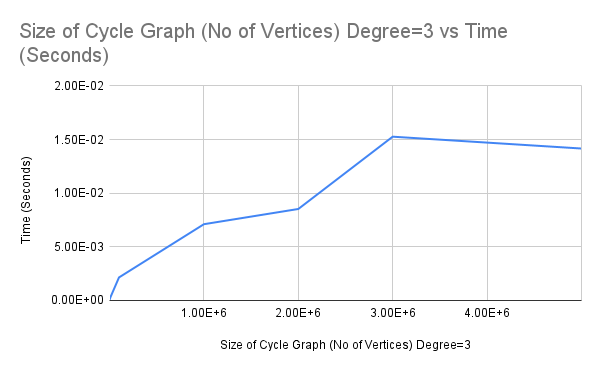
\includegraphics[width=.50\textwidth]{Size of Cycle Graph (No of Vertices) Degree=3 vs Time (Seconds).png}\hfill
    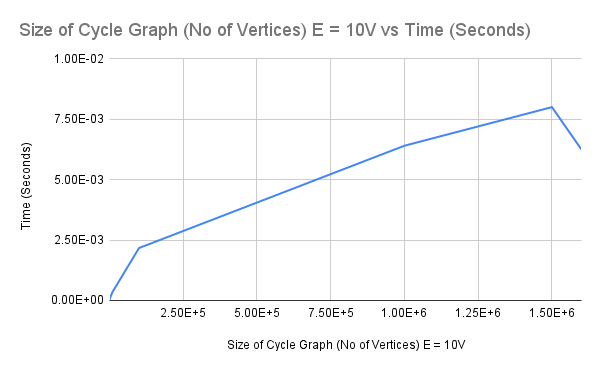
\includegraphics[width=.50\textwidth]{Size of Cycle Graph (No of Vertices) E = 10V vs Time (Seconds).png}\hfill
    \\[\smallskipamount]
    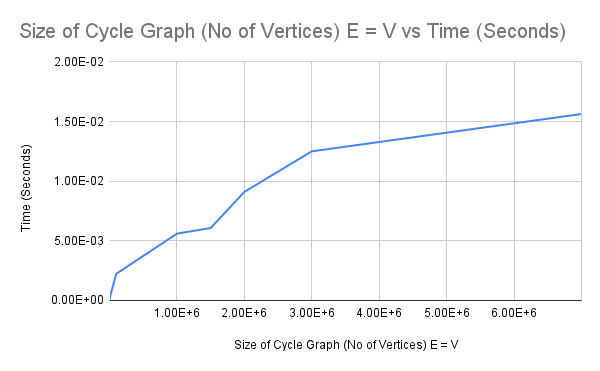
\includegraphics[width=.50\textwidth]{Size of Cycle Graph (No of Vertices) E = V vs Time (Seconds).png}\hfill
    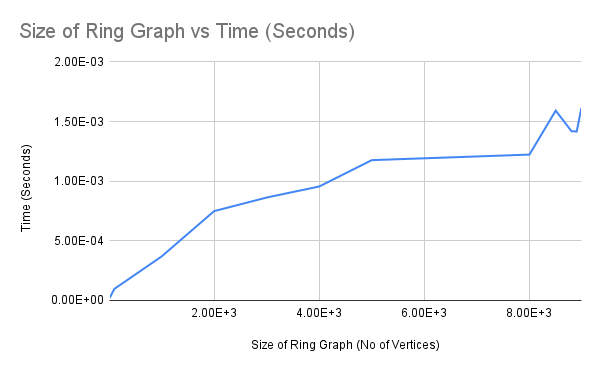
\includegraphics[width=.50\textwidth]{Size of Ring Graph vs Time (Seconds).png}\hfill
    \caption{Graphical analysis of running time and complexity of the cycle finding algorithm}\label{fig:findcycle}
\end{figure}
\section*{Problem 2}
\subsection*{Minimum Spanning Tree for sparse graphs [50]} 
\subsubsection*{Solution}
\textbf{Algorithm}\\
The algorithm for developing a minimum spanning three for a sparse graph ($|E|=O(|V|+8)$) using the cycle finding algorithm from the first problem. As there are very few edges, we run the finding algorithm to find a cycle where we remove the max weighted edge. After that we run the find cycle algorithm just that many times such that there are only $|V|-1$ edges left. The final result left is the minimum spanning tree. The modified algorithm is shown as remove cycle algorithm in Algorithm~\ref{alg:main2}.\\ This algorithm works because of the red-rule i.e. marking an edge in a cycle with max weight with red-color and discarding it for each $findcycle$ call and then remove all the red edges to get the final minimum spanning tree.
\begin{algorithm}
\caption{Function for removing the max weighted cycle in the graph to form MST}
\label{alg:main2}
\begin{algorithmic}[1]
\State \textbf{Input:} Graph\ $G$ with $|V|$ vertices and $|E|$ edges. Global $cycleList[]$.
\State \textbf{Output:} Removes the highest weghted edge from the cycle found.
\Function{RemoveCycle}{$G$}:
\State $cycle\leftarrow FALSE;$
 \For {nodes $v \in V(G)$}
\If {$visited[v]\ = FALSE$}
\If {$FindCycleHelper(v, visited[], -1) = TRUE$}
\State $cycle\leftarrow TRUE$;
\State break;
\EndIf
\EndIf
\EndFor
\If{$cycle = TRUE$}
\State $root \leftarrow cycleList[-1]$;
\For {nodes $v\ in\ cycleList$ from the end}
\State Remove the edge $e$ from Graph $G$, such that W(e) is max of all the edges in the cycle
\EndFor
\EndIf
\State \Return;
\EndFunction

\State Call $RemoveCycle(G)\ (|E|-|V|+1)$ times
\State Print remaining edges gives the minimum spanning three
\end{algorithmic}
\end{algorithm}

\textbf{Analysis}\\
\textit{Proof of Correctness}\\
The algorithm always finds the MST for Sparse Graphs [$|E| = O(|V|+8)$].
Assuming that the Graph has at most $|V|+8$ edges and at least $|V|$ edges.\\
\textbf{Proof:} This can be proved using a modified red-rule. The red-rule suggests that: Let C be a cycle with no red edges. Select an uncolored
edge of C of max weight and color it red~\cite{tarjan1983data}.
Now, we apply the red-rule after finding a cycle and discard that edge and run the cycle finding algorithm again and apply the red-rule again till we color $|E|-|V|+1$ edges  [$\because$ We want $|V|-1$ edges to be uncolored for the Graph to form a MST and we have $|E|=O(|V|+8)$ edges]. Now, the remaining edges form the Minimum Spanning Tree. Essentially, in each cycle finding, we remove an edge i.e. remove a cycle and thus we remove enough edges to form a tree from the given Sparse Graph. We color the edge with a constraint such that every time we color the max-weight edge. By doing this we ensure that we remove all the max-weighted edges from the graph while keeping the graph connected and remove all the unwanted cycle in the process. Thus, the algorithm always finds the MST. This works for Sparse Graph constraints given in the question because there are at most $|E|-|V|+1$ cycles, and thus we have to apply this modified rule only constant amount of times.\\\\
\textit{Running Time}\\
The running time of the proposed algorithm is $O(|E|)$, when we use. the adjacency list representation of the Sparse Graph $G$.\\
\textbf{Proof:} The remove cycle algorithm essentially finds cycle and removes the max weight edge using DFS; and thus it takes $O(|E|+|V|)$ time to run as discussed in section 1. Now, we run this algorithm a maximum of $O(|E|-|V|+1)$ times to remove enough max-weight edges to form the minimum spanning tree. In our case, $|E| = O(|V|+8)$, thus the remove cycle algorithm runs a max of $O(|V|-|V|+8+1) = O(9)$ times, and each time the cycle finding algorithm runs for $O(|E|+|V|) = O(2*|V|+8)$. Thus, the final runtime of the algorithm is $O(9*(2*|V|+8)) \approx O(|V|)$. \\
Figure~\ref{fig:mst} shows the analysis of running time as a function of size of the graph. The evaluation is done for the same in the following way. 
\begin{enumerate}
    \item By varying the no. of edges of the graph in the range ${|V|,|V|+8}$ and assigning the weights randomly to the edges between the range ${100, 500}$. The \textit{LinearGraphGenerator}~\cite{10.1145/3381449, kim2003generating} constructor was used to generate a graph with $|V|-1$ edges and the rest of the edges were added randomly to the graph to create the final graph.
\end{enumerate}
It is clear from the graph that the algorithm's run time follows linear-time complexity  (\textit{$O(|V|)$}) for increasing size of the graph.
\begin{figure}[htp]
\begin{center}
    \includegraphics[width=0.6\textwidth]{Size of Graph E = V + rand{0,8},W={100, 500} vs Time (Seconds).png}
    \caption{Graphical analysis of running time and complexity of the minimum spanning tree algorithm}\label{fig:mst}
\end{center}
\end{figure}
\clearpage
\section*{Guide to Code}
Both the codes were written in Java language. 
\subsubsection*{Steps}
\begin{enumerate}
    \item Download and Install JDK 11+ on your system using the following link:~\href{https://www.oracle.com/java/technologies/downloads/}{JDK}
    \item Create new java projects one-by-one and use the $findcycle.java$ and $mst.java$ for problem 1 and problem 2.
    \item Download and Add the JgraphT dependency to the java project using the following link:~\href{https://jgrapht.org/#download}{JGraphT}.
    \item Run the java projects and interactively give input according to the prompt.
\end{enumerate}
\textit{$^*$Tip: Use VS code and Java extensions for easy install and execution.}\\
\\The testing of both the codes was done using unit-test cases. Evaluation of the code in-terms of time was done using the $nanoTime()\ package$ of java. 
\bibliographystyle{plain}
\bibliography{main}
\end{document}
